\documentclass[tikz,border=4pt]{standalone}
\usepackage[T1]{fontenc}
\usepackage{helvet}
\renewcommand{\familydefault}{\sfdefault}
\usetikzlibrary{arrows.meta,positioning,shapes.geometric,fit}
\definecolor{ink}{HTML}{1F2937}
\definecolor{muted}{HTML}{64748B}
\definecolor{line}{HTML}{94A3B8}
\definecolor{blue}{HTML}{D9EAFE}
\definecolor{green}{HTML}{DCFCE7}
\definecolor{amber}{HTML}{FEF3C7}
\definecolor{violet}{HTML}{EDE9FE}
\definecolor{rose}{HTML}{FFE4E6}
\definecolor{panel}{HTML}{F8FAFC}
\begin{document}
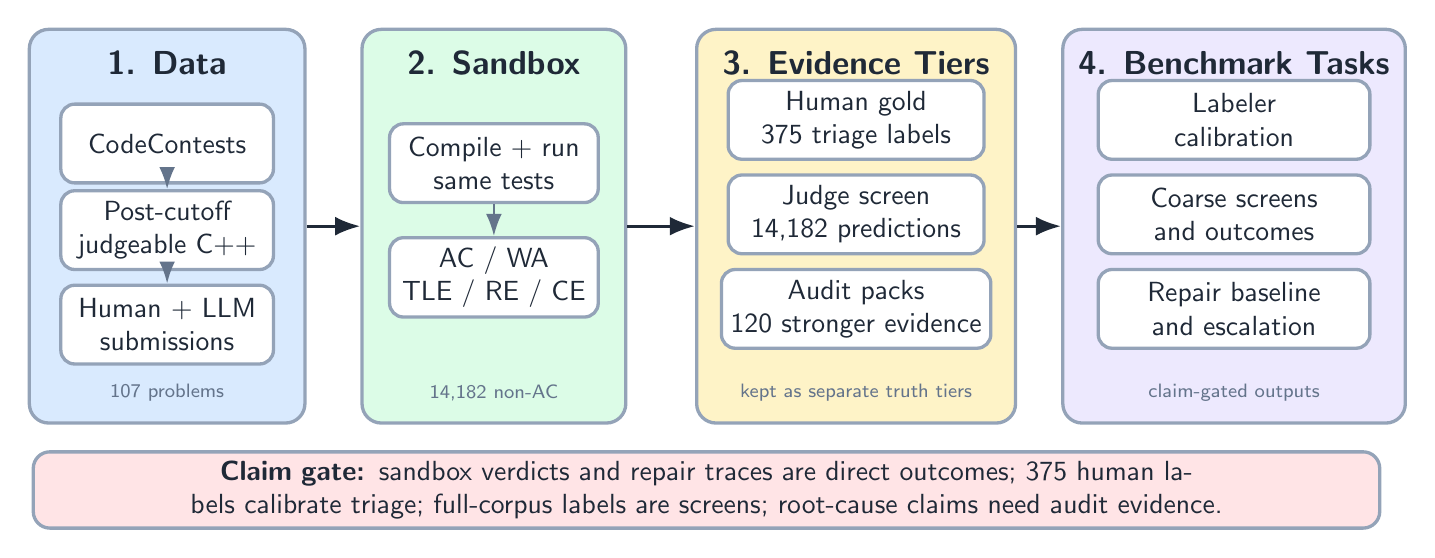
\begin{tikzpicture}[
  font=\sffamily,
  box/.style={rounded corners=5pt, draw=line, very thick, fill=white,
    minimum height=1.0cm, align=center, text=ink},
  panelbox/.style={rounded corners=7pt, draw=line, very thick, fill=panel,
    minimum height=5.0cm, align=center, text=ink},
  title/.style={font=\sffamily\bfseries\large, text=ink},
  small/.style={font=\sffamily\small, text=ink},
  tiny/.style={font=\sffamily\scriptsize, text=muted},
  arrow/.style={-{Latex[length=3.2mm,width=2.4mm]}, very thick, draw=ink},
  softarrow/.style={-{Latex[length=2.8mm,width=2.0mm]}, thick, draw=muted}
]

\node[panelbox, minimum width=3.5cm, fill=blue] (p1) at (0,0) {};
\node[title] at (p1.north) [yshift=-0.45cm] {1. Data};
\node[box, minimum width=2.7cm] (cc) at ([yshift=1.05cm]p1.center) {CodeContests};
\node[box, minimum width=2.7cm] (filter) at ([yshift=-0.05cm]p1.center) {Post-cutoff\\judgeable C++};
\node[box, minimum width=2.7cm] (subs) at ([yshift=-1.25cm]p1.center) {Human + LLM\\submissions};
\draw[softarrow] (cc) -- (filter);
\draw[softarrow] (filter) -- (subs);
\node[tiny] at ([yshift=-2.12cm]p1.center) {107 problems};

\node[panelbox, minimum width=3.35cm, fill=green] (p2) at (4.15,0) {};
\node[title] at (p2.north) [yshift=-0.45cm] {2. Sandbox};
\node[box, minimum width=2.65cm] (judge) at ([yshift=0.80cm]p2.center) {Compile + run\\same tests};
\node[box, minimum width=2.65cm] (verdict) at ([yshift=-0.65cm]p2.center) {AC / WA\\TLE / RE / CE};
\draw[softarrow] (judge) -- (verdict);
\node[tiny] at ([yshift=-2.12cm]p2.center) {14,182 non-AC};

\node[panelbox, minimum width=4.05cm, fill=amber] (p3) at (8.75,0) {};
\node[title] at (p3.north) [yshift=-0.45cm] {3. Evidence Tiers};
\node[box, minimum width=3.25cm] (gold) at ([yshift=1.35cm]p3.center) {Human gold\\375 triage labels};
\node[box, minimum width=3.25cm] (screen) at ([yshift=0.15cm]p3.center) {Judge screen\\14,182 predictions};
\node[box, minimum width=3.25cm] (audit) at ([yshift=-1.05cm]p3.center) {Audit packs\\120 stronger evidence};
\node[tiny] at ([yshift=-2.12cm]p3.center) {kept as separate truth tiers};

\node[panelbox, minimum width=4.35cm, fill=violet] (p4) at (13.55,0) {};
\node[title] at (p4.north) [yshift=-0.45cm] {4. Benchmark Tasks};
\node[box, minimum width=3.45cm] (cal) at ([yshift=1.35cm]p4.center) {Labeler\\calibration};
\node[box, minimum width=3.45cm] (coarse) at ([yshift=0.15cm]p4.center) {Coarse screens\\and outcomes};
\node[box, minimum width=3.45cm] (repair) at ([yshift=-1.05cm]p4.center) {Repair baseline\\and escalation};
\node[tiny] at ([yshift=-2.12cm]p4.center) {claim-gated outputs};

\draw[arrow] (p1.east) -- (p2.west);
\draw[arrow] (p2.east) -- (p3.west);
\draw[arrow] (p3.east) -- (p4.west);

\node[box, fill=rose, rounded corners=6pt, minimum width=17.1cm, text width=16.55cm,
  minimum height=0.95cm]
  (gate) at (6.85,-3.35)
  {\textbf{Claim gate:} sandbox verdicts and repair traces are direct outcomes;
  375 human labels calibrate triage; full-corpus labels are screens; root-cause claims need audit evidence.};

\end{tikzpicture}
\end{document}
